%pour la mise en page
\documentclass[a4paper,10pt]{report}
\usepackage[utf8]{inputenc}

%pour les figures
\usepackage{float}
\usepackage{graphicx}

\usepackage[top=3cm, bottom=3cm, left=3cm, right=3cm]{geometry}

\renewcommand{\chaptername}{Chapitre}
\renewcommand{\contentsname}{Table des matières}
\renewcommand{\listfigurename}{Table des Figures}

\usepackage{fancyhdr}
\pagestyle{fancy}
\renewcommand\headrulewidth{1pt}
\fancyhead[L]{Rapport de projet LO21}
\fancyhead[R]{\leftmark}
\renewcommand\footrulewidth{1pt}
\fancyfoot[L]{UTC}
\fancyfoot[C]{\thepage}
\fancyfoot[R]{Beaudou Camille / Marlow Justine}

\makeatletter
\let\ps@plain=\ps@fancy
\makeatother

\begin{document}
\title{Rapport de projet LO21}
\author{Camille Beaudou et Justine Marlow}
\date{Printemps 2017}
\maketitle
\addcontentsline{toc}{chapter}{Table des matières}
\tableofcontents
%\newpage
%\addcontentsline{toc}{chapter}{Table des figures}
%\listoffigures
\newpage

\chapter{Description de l'architecture}
\section{Présentation globale}
Nous avons décidé, pour répondre au cahier des charges posé par le sujet du projet \textit{PluriNotes} d'implémenter l'ensemble des classes de l'architecture décrite dans l'UML (\ref{UML_global}).
\begin{center}
\begin{figure}[H]
\caption{UML : Architecture globale du projet}
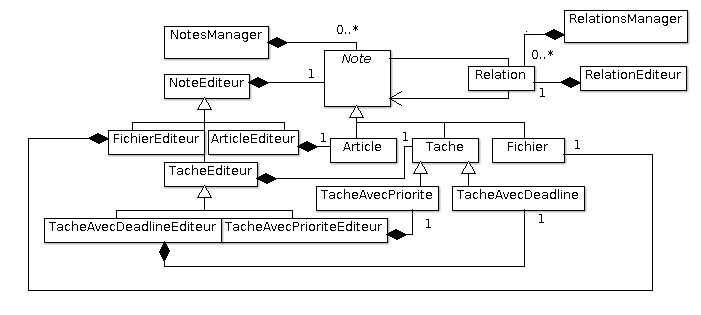
\includegraphics[width=\textwidth]{UML_global.png}
\label{UML_global}
\end{figure}
\end{center}
Cet UML est volontairement constitué d'uniquement les noms des classes, par souci de clarté et de lisibilité. Ces différentes classes, que nous expliciterons dans la suite de ce rapport, peuvent être classées dans différentes catégories qui guideront notre description du projet.
\begin{itemize}
\item La classe Note et ses classes filles
\item La classe Relation
\item Les classes NotesManager et RelationsManager
\item Les classes Editeurs
\end{itemize}
Nous allons détailler pour chacune de ses catégories les diagrammes UML des classes et les choix d'implémentations que nous avons réalisé.

\section{Présentation de la classe Note et de ses classes filles}
Nous avons choisi d'implémenter les classes \textit{Note}, \textit{Article}, \textit{Tache}, \textit{TacheAvecPriorite}, \textit{TacheAvecDeadline} et \textit{Fichier} en utilisant l'héritage. Nous avons donc suivi l'UML (\ref{UML_note}).
\begin{center}
\begin{figure}[H]
\caption{UML : Architecture de la classe Note et de ses classes filles}
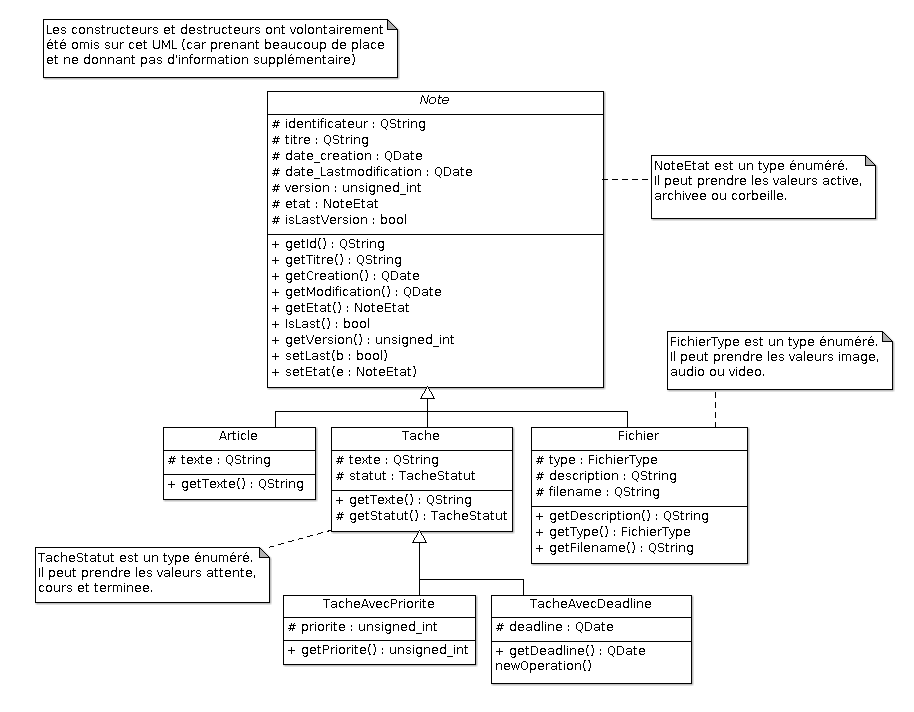
\includegraphics[width=\textwidth]{UML_note.png}
\label{UML_note}
\end{figure}
\end{center}

\subsection{Abstraction de la classe Note}
Nous avons choisi d'implémenter la classe \textit{Note} comme une classe abstraite. En effet, compte tenu du sujet du projet, nous avons considérer qu'une \textit{note} était soit un \textit{article}, soit une \textit{tâche} (ou \textit{tâche avec priorité} ou \textit{tâche avec deadline}), soit un \textit{fichier}. En effet, la possibilité de gérer une simple \textit{note}, autrement dit un \textit{id} et un \textit{titre} ne nous a pas paru intéressante ni même utile.

\subsection{Regroupement des images, des enregistrements audio et vidéo dans la classe Fichier}
Comme les images, enregistrements audio et vidéo sont tous trois caractérisés par une description et un fichier, nous avons décidé de les regrouper sous une seule et même classe appelée \textit{Fichier}.

\subsection{Gestion des versions}
Pour gérer les différentes versions d'une note, nous avons décider qu'à chaque modification d'un objet \textit{note}, un nouvel objet \textit{note} avec les nouvelles valeurs des attributs est créé. Les attributs \textit{id} et \textit{date\_ creation} ne changent pas (ainsi plusieurs objets \textit{note} peuvent avoir le même \textit{id} à la condition qu'il s'agisse de deux versions d'une même \textit{note}). Les attributs \textit{isLast} et \textit{version} sont gérés par l'application.

\subsection{Attributs protected et constructeurs}
Les attributs de ces différentes classes sont tous dans le domaine \textit{protected} pour permettre aux classes filles d'accéder à ces attributs. Il a été choisi de ne pas faire apparaître les constructeurs (ni les destructeurs) dans cet UML. Toutefois il est important de stipuler qu'ils sont également dans le domaine \textit{protected} afin que la gestion de la création et de la destruction d'objet \textit{Note} ne puissent se faire que via le \textit{NotesManager} (cf section \ref{NotesManager & RelationsManager}).

\section{Présentation de la classe Relation}
Nous avons implémenter la classe \textit{Relation} en tant que classe-association : elle permet d'associer des objets \textit{Note} entre eux. Ainsi, une relation a pour attribut un tableau bi-dimensionnel de \textit{Note*}. Nous avons donc suivi les UML (\ref{UML_relation}) (à nouveau, nous avons préféré ne pas indiquer les constructeurs et destructeurs comme ils n'apportent pas plus d'information et par souci de clarté et de lisibilité).
\begin{center}
\begin{figure}[H]
\caption{UML : Architecture de la classe Relation}
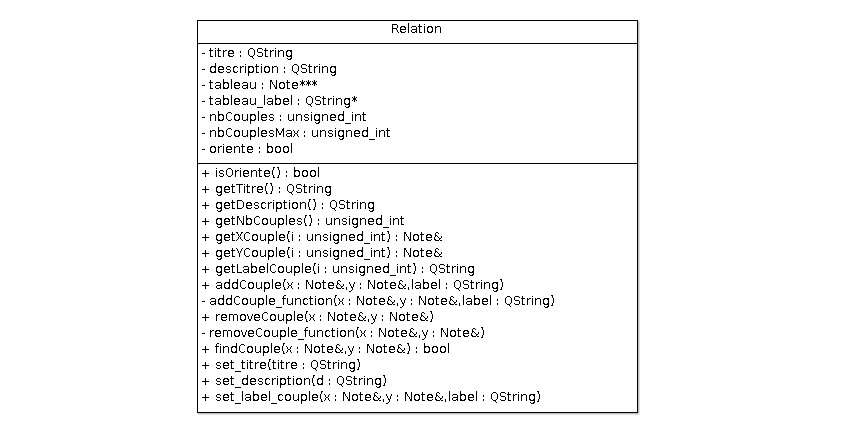
\includegraphics[width=\textwidth]{UML_relation.png}
\label{UML_relation}
\end{figure}
\end{center}

\section{Présentation des classes NotesManager et RelationsManager}
\label{NotesManager & RelationsManager}
Les classes \textit{NotesManager} et \textit{RelationsManager} ont été implémentées dans le but de gérer totalement les objets dont elles sont responsables, c'est à dire leur création, leur utilisation et leur destruction. Ainsi, les constructeurs et destructeurs de la classe \textit{Note} et ses classes filles (resp. \textit{Relation}) sont dans le domaine \textit{protected} et il existe une amitié entre ses classes et la classe NotesManager (resp. \textit{RelationsManager}). Nous avons donc suivi les UML (\ref{UML_notemanager}) et (\ref{UML_relationmanager}).
\begin{center}
\begin{figure}[H]
\caption{UML : Architecture de la classe NotesManager}
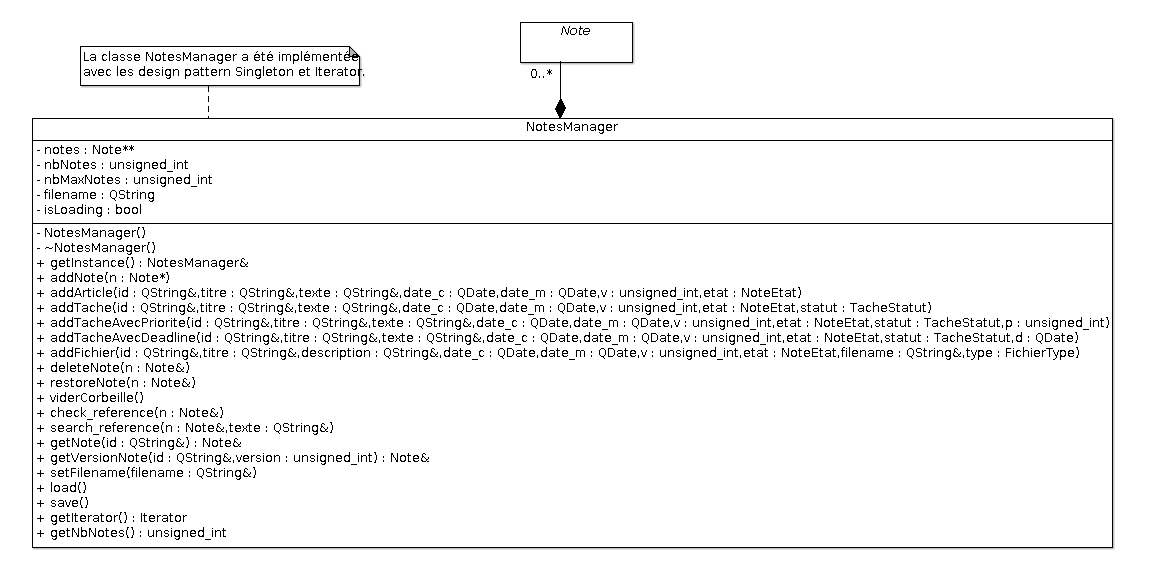
\includegraphics[width=\textwidth]{UML_notemanager.png}
\label{UML_notemanager}
\end{figure}
\end{center}

\begin{center}
\begin{figure}[H]
\caption{UML : Architecture de la classe RelationsManager}
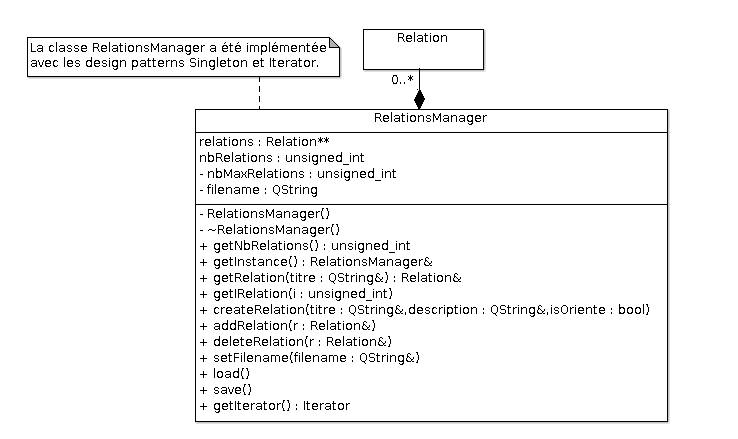
\includegraphics[width=\textwidth]{UML_relationmanager.png}
\label{UML_relationmanager}
\end{figure}
\end{center}

\section{Présentation des classes Editeur}

\chapter{Possibilité d'évolution de l'architecture}
\begin{itemize}
\item Extension à d'autres types de note
\end{itemize}

\end{document}